\chapter{Coatings for CAST}
Afte the launch of NuSTAR, the X-ray optics group at DTU Space was invited to participate in the creation of an X-ray optic for the CAST solar axion helioscope. CAST is an experiment at CERN that looks for the hypothetical axion particle which is a solution to the charge-parity (CP) problem of the standard model in particle physics. If the axion exist, it is also some or all of the dark matter in the universe. It was assumed that the technology from NuSTAR could be leveraged and therefore use spare glass to make a cheap and relatively simple X-ray optic.

The optic was designed between summer 2012 and summer 2014. Production, assembly, installation and alignment with CAST was done during summer 2014 in cooperation with University of Zaragoza in Spain and Lawrence Livermore National Lab in the US. In this chapter the reader will find a description of the whole process from start to finish.

\section{The CAST instrument}

The axion is an ultra-light particle that is formed from the interaction of a photon with an electromagnetic field, called the Primakoff effect. So the main sources of the particle would be from inside stars, and from Earth the best nearby source will of course be the Sun. The axion is weakly interacting so in order to detect it, CAST uses a strong magnet to convert the axion back to a photon again by the Primakoff effect. The photons subsequently hit a detector.

\begin{figure}[htbp]
  \centering
    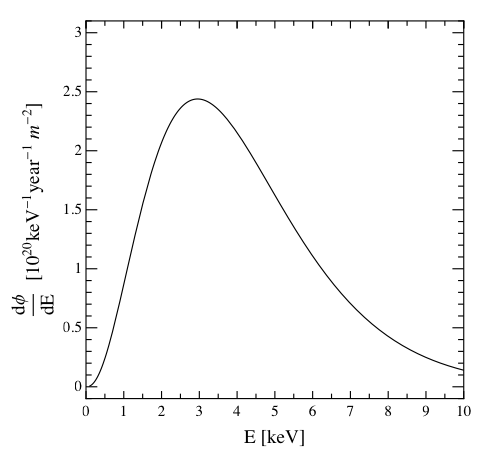
\includegraphics[height=6cm]{figures/cast/axion_spectrum.png}
  \caption{}
  \label{fig:axion_spectrum}
\end{figure}

The spectrum of X-rays from axions can be seen in figure \ref{fig:axion_spectrum}. It is relatively low energy X-rays with a peak around 3 keV and a shape similar to the black-body radiation spectrum.

\begin{figure}[htbp]
  \centering
    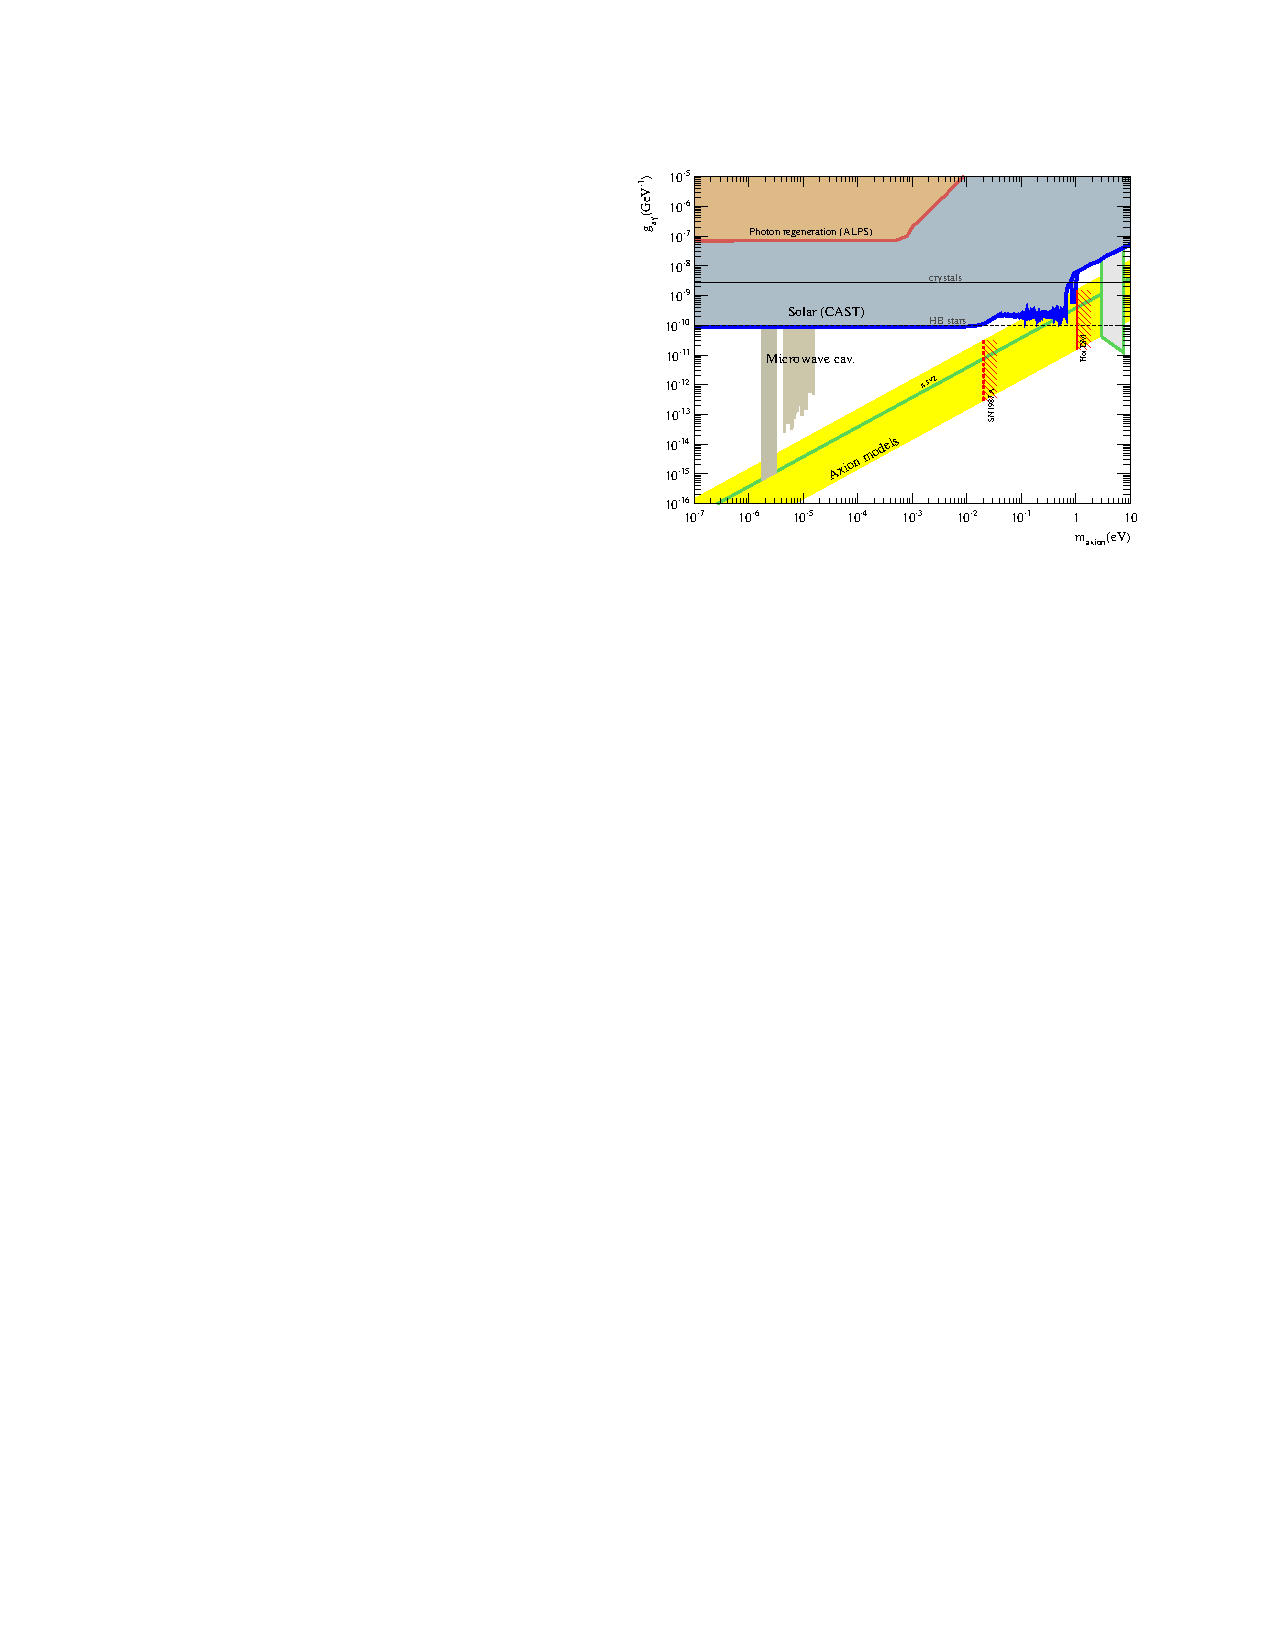
\includegraphics[height=6cm]{figures/cast/axion_search_cast.pdf}
  \caption{}
  \label{fig:axion_search_cast}
\end{figure}

From theory, the expected mass of the axion is between $10^{-7}$-$1$ eV. In figure \ref{fig:axion_search_cast} the search area can be seen as the axion-photon coupling constant, \gay, as a function of the axion mass, \maxion. The yellow line represents the area where we expect to see the axion if all dark matter in the universe consists of axion particles with the same \maxion\ and \gay. The CAST helioscope is by 2014 the most comprehensive axion search, and has set an experimental upper limit of

\begin{eqnarray}
\gaymath \leq 2 \cdot 10^{-10} \textrm{ GeV}^{-1}.
\end{eqnarray}

% \begin{figure}
% \centering
% \begin{minipage}{.5\textwidth}
%   \centering
%   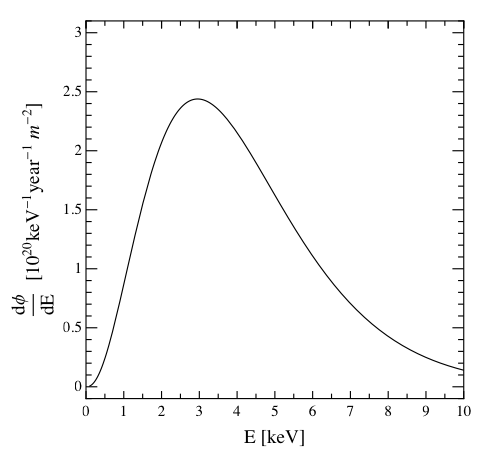
\includegraphics[height=4.6cm]{figures/cast/axion_spectrum.png}
%   \captionof{figure}{A figure}
%   \label{fig:axion_spectrum}
% \end{minipage}%
% \begin{minipage}{.5\textwidth}
%   \centering  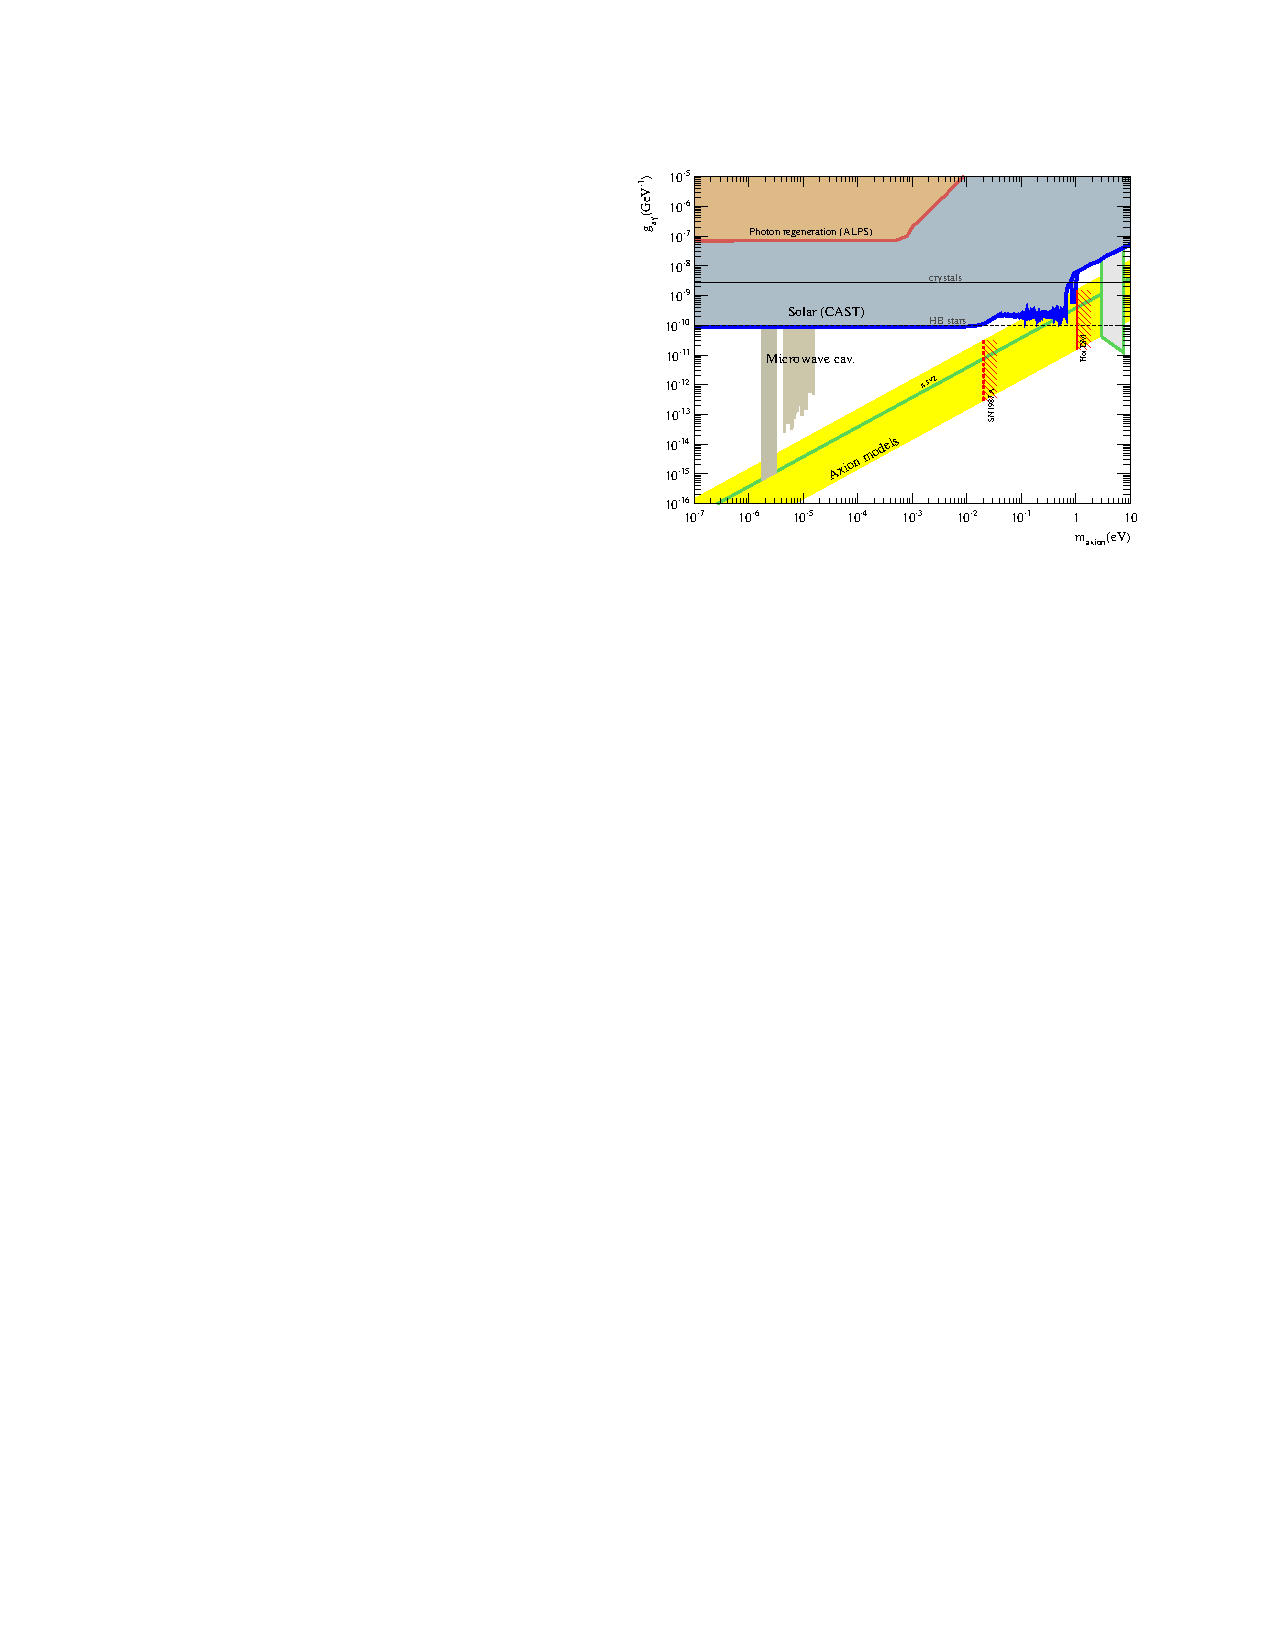
\includegraphics[width=\linewidth]{figures/cast/axion_search_cast.pdf}
%   \captionof{figure}{Another figure}
%   \label{fig:axion_search_cast}
% \end{minipage}
% \end{figure}

The CAST experiment is largely made from spare parts of other projects at CERN and other research institutions. The magnet is one of three prototype superconducting dipole magnets from the Large Hadron Collider. It is designed to transport particles in two directions inside a strong magnetic field, so it has two bores inside with diameters of 45 mm. As can be seen in the picture of the CAST instrument (figure \ref{fig:cast_instrument}), the magnet is able to pitch and yaw up to a limit. That makes it possible to follow the sun as it comes up with one end and as it goes down with the other end. Since the axion does not interact with matter, detectors are placed at both ends of the magnet and at both boreholes, so two detectors can be used at sunrise and two at sunset.

\begin{figure}[htbp]
  \centering
    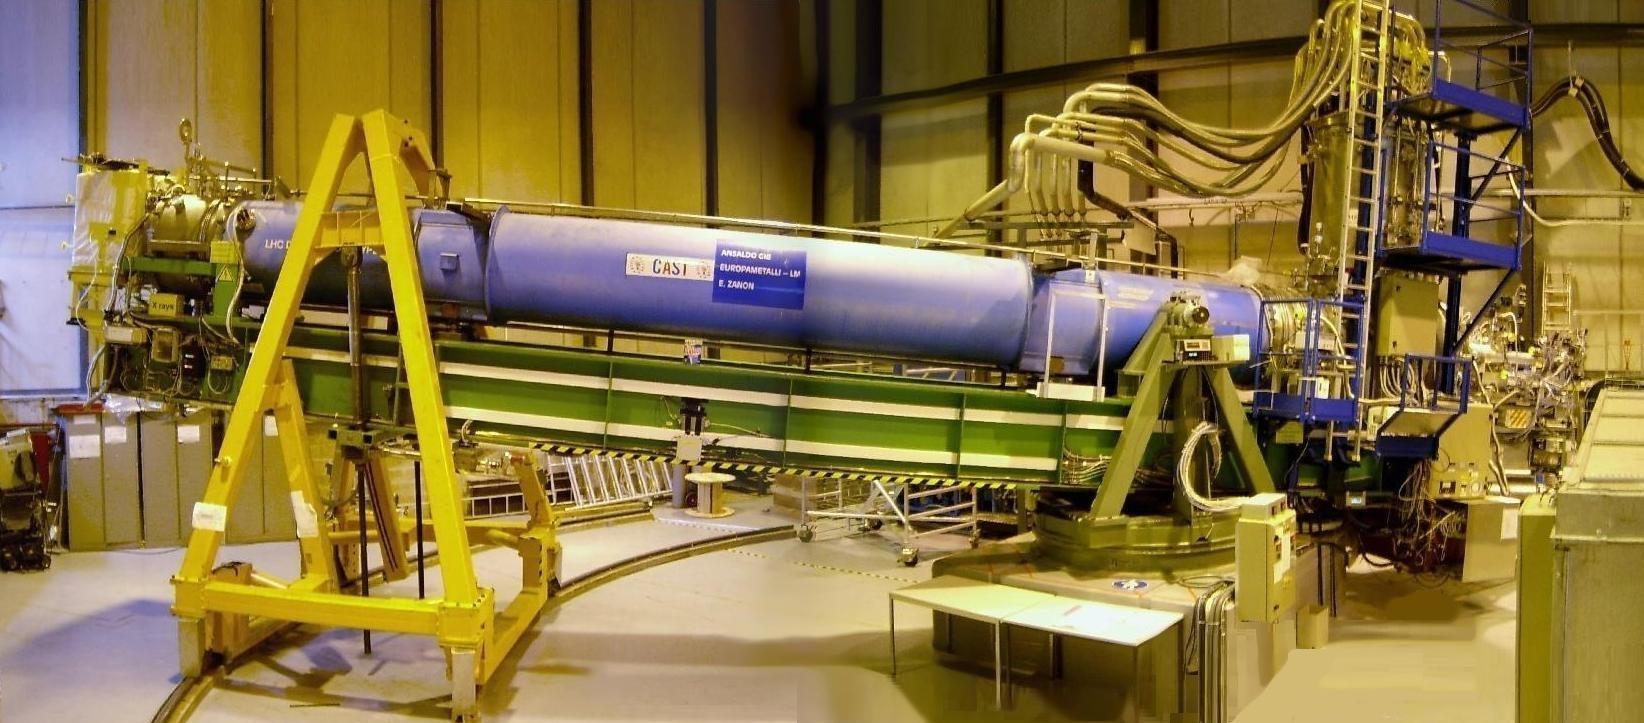
\includegraphics[height=5cm]{figures/cast/cast_instrument.jpg}
  \caption{}
  \label{fig:cast_instrument}
\end{figure}

!!!!!!!Something about Micromegas detectors!!!!!

CAST has been doing axion searches since 2002 and the experiment continually improves and reiterates the equipment to get higher sensitivity. One major problem is to get a high enough signal-to-noise ratio, the majority of the noise coming from background radiation from the ground, the materials and also cosmic rays.

The detectors covers the entire area of each bore opening, so are relatively large. Detector size is proportional to the background radiation, so it makes sense to have smaller detectors. By using X-ray optics, the X-ray photons can be focused into a detector area of only a fraction of the previous. This will significantly increase the signal-to-noise ratio and will let the CAST helioscope search for the axion in new areas.

\section{Developing an optic for CAST}
One major concern in making an X-ray optic from NuSTAR glass for the CAST helioscope is the limited space available. The optic would have to fit on the end of the magnet nearest the wall, which leaves only about 2 meters for optic, detector and the focal length between the two. Another problem is the small bore opening of only 45 mm, which is smaller than the inner radius of the NuSTAR telescopes. Both of those problems can be solved by realising that the optic would not require imaging capability and the axion spectrum is of relatively low energies.

!!!Diagram of CAST exp. hall from top, shows the limited space!!!

\begin{figure}[htbp]
  \centering
    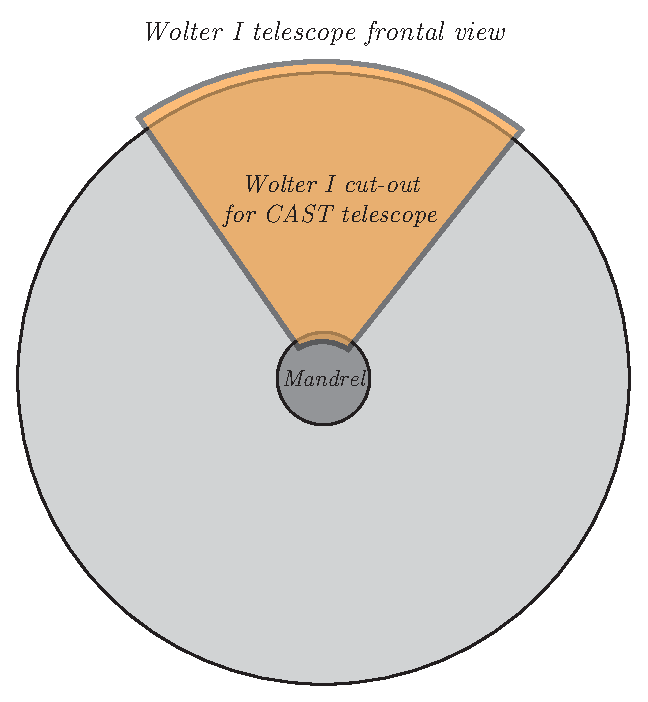
\includegraphics[height=6cm]{figures/cast/wolter1-cutout.eps}
  \caption{}
  \label{fig:wolter1-cutout}
\end{figure}

By using only 1/6 of the Wolter I radial reflective area, a pie-slice (figure \ref{fig:wolter1-cutout}), two stacks of mirrors can be used to reflect X-rays to one side. The stack only needs to be high enough to cover the bore opening, but each mirror should also be wide enough. The NuSTAR glass are made in 60\degr\ segments for the inner radii and 30\degr\ segments for the outer radii.

\subsection{Optic geometry considerations}
The geometry of the optic was calculated using the following equation for a Wolter I optic:

\begin{eqnarray}\label{eq:wolter}
  \tan(4\alpha) = \frac{\rho}{f},
\end{eqnarray}

where $\alpha$ is the angle of reflection of each mirror, $f$, is the focal length and $\rho$ is the radius between center of optic and the midpoint between parabolic and hyperbolic mirror (figure \ref{fig:wolter1-diagram}). The center of the bore will need an off-set with the focal plane of the telescope, given by $d$, which is the radius of the bore, $r_{\text{bore}}$, plus the minimum radius of a NuSTAR optic, $r_{\text{min}}$ (figure \ref{fig:optic_and_bore}). The length of the NuSTAR mirrors is $l = 225$ mm.

\begin{figure}
\centering
\begin{minipage}{.5\textwidth}
  \centering
  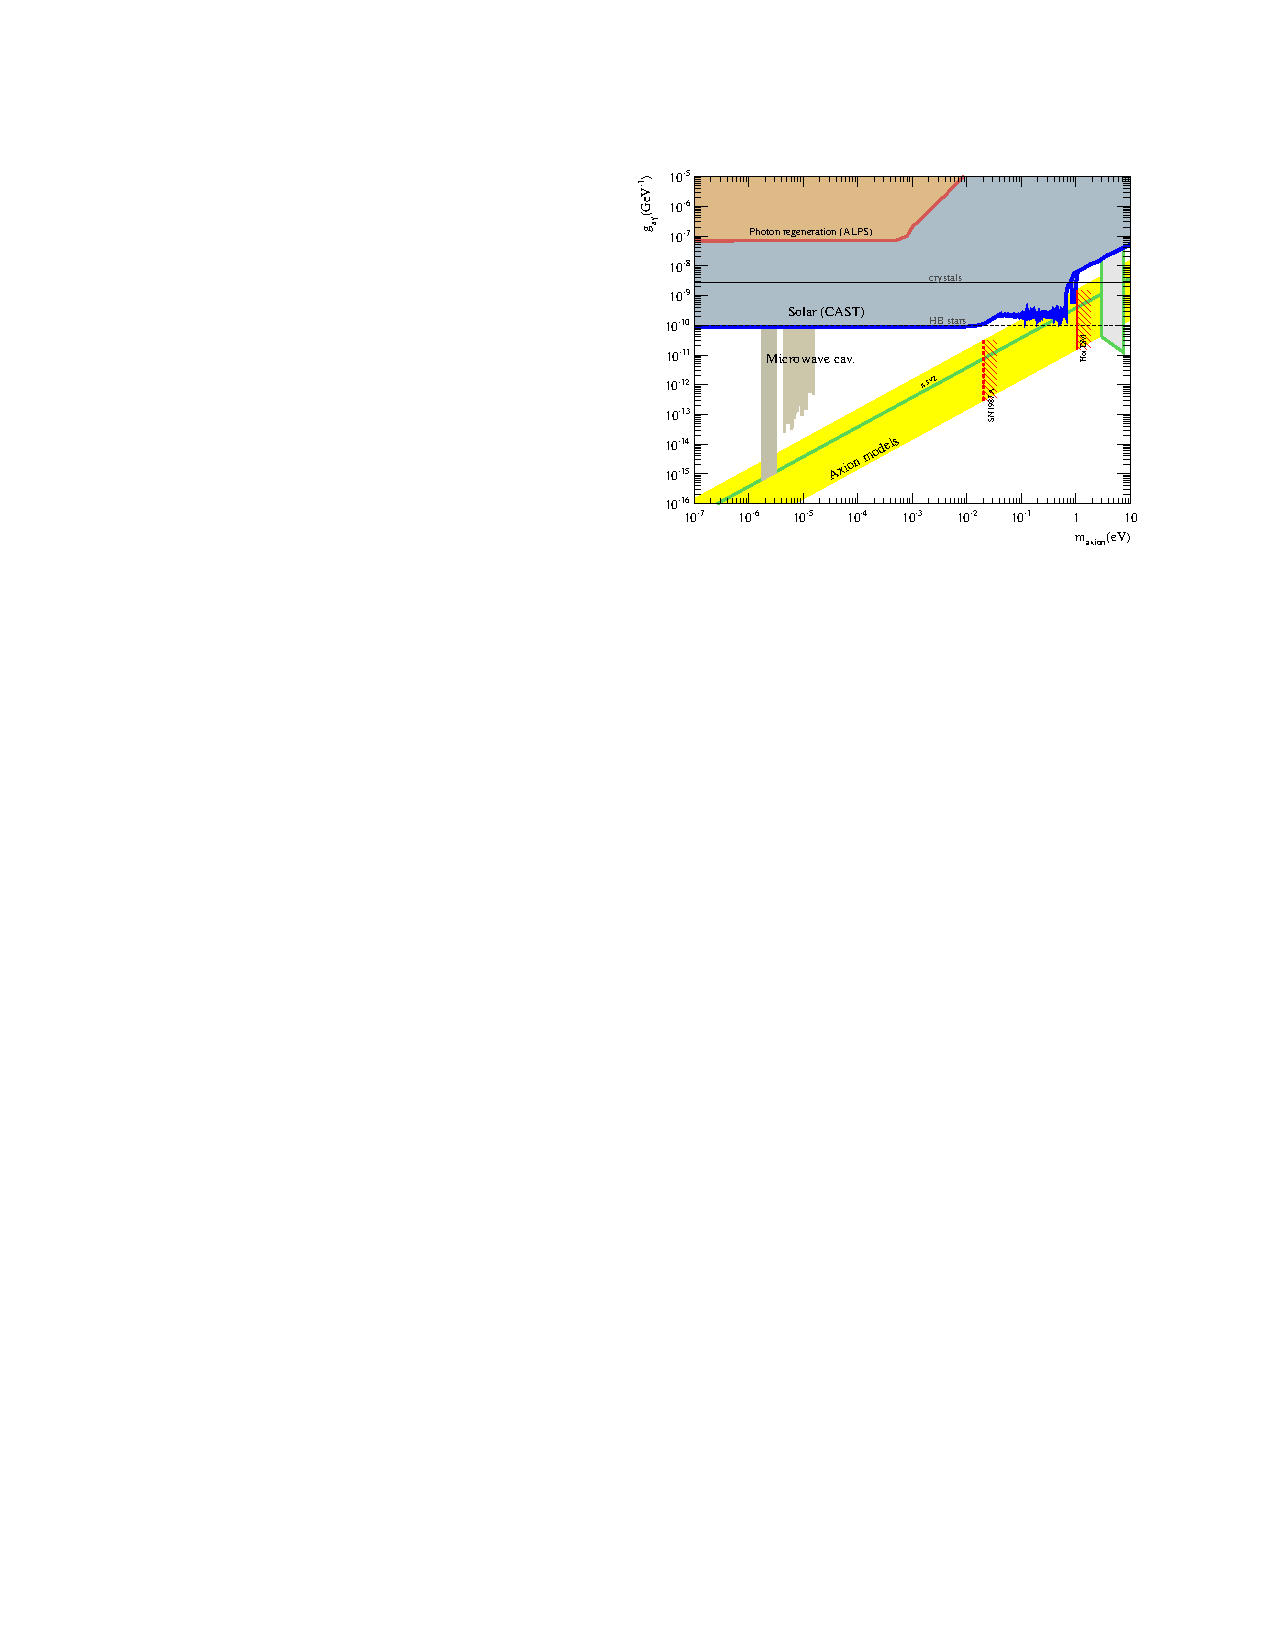
\includegraphics[width=\linewidth]{figures/cast/axion_search_cast.pdf}
  \captionof{figure}{Diagram of wolter I from side.R1-R5 designated.}
  \label{fig:wolter1-diagram}
\end{minipage}%
\begin{minipage}{.5\textwidth}
  \centering  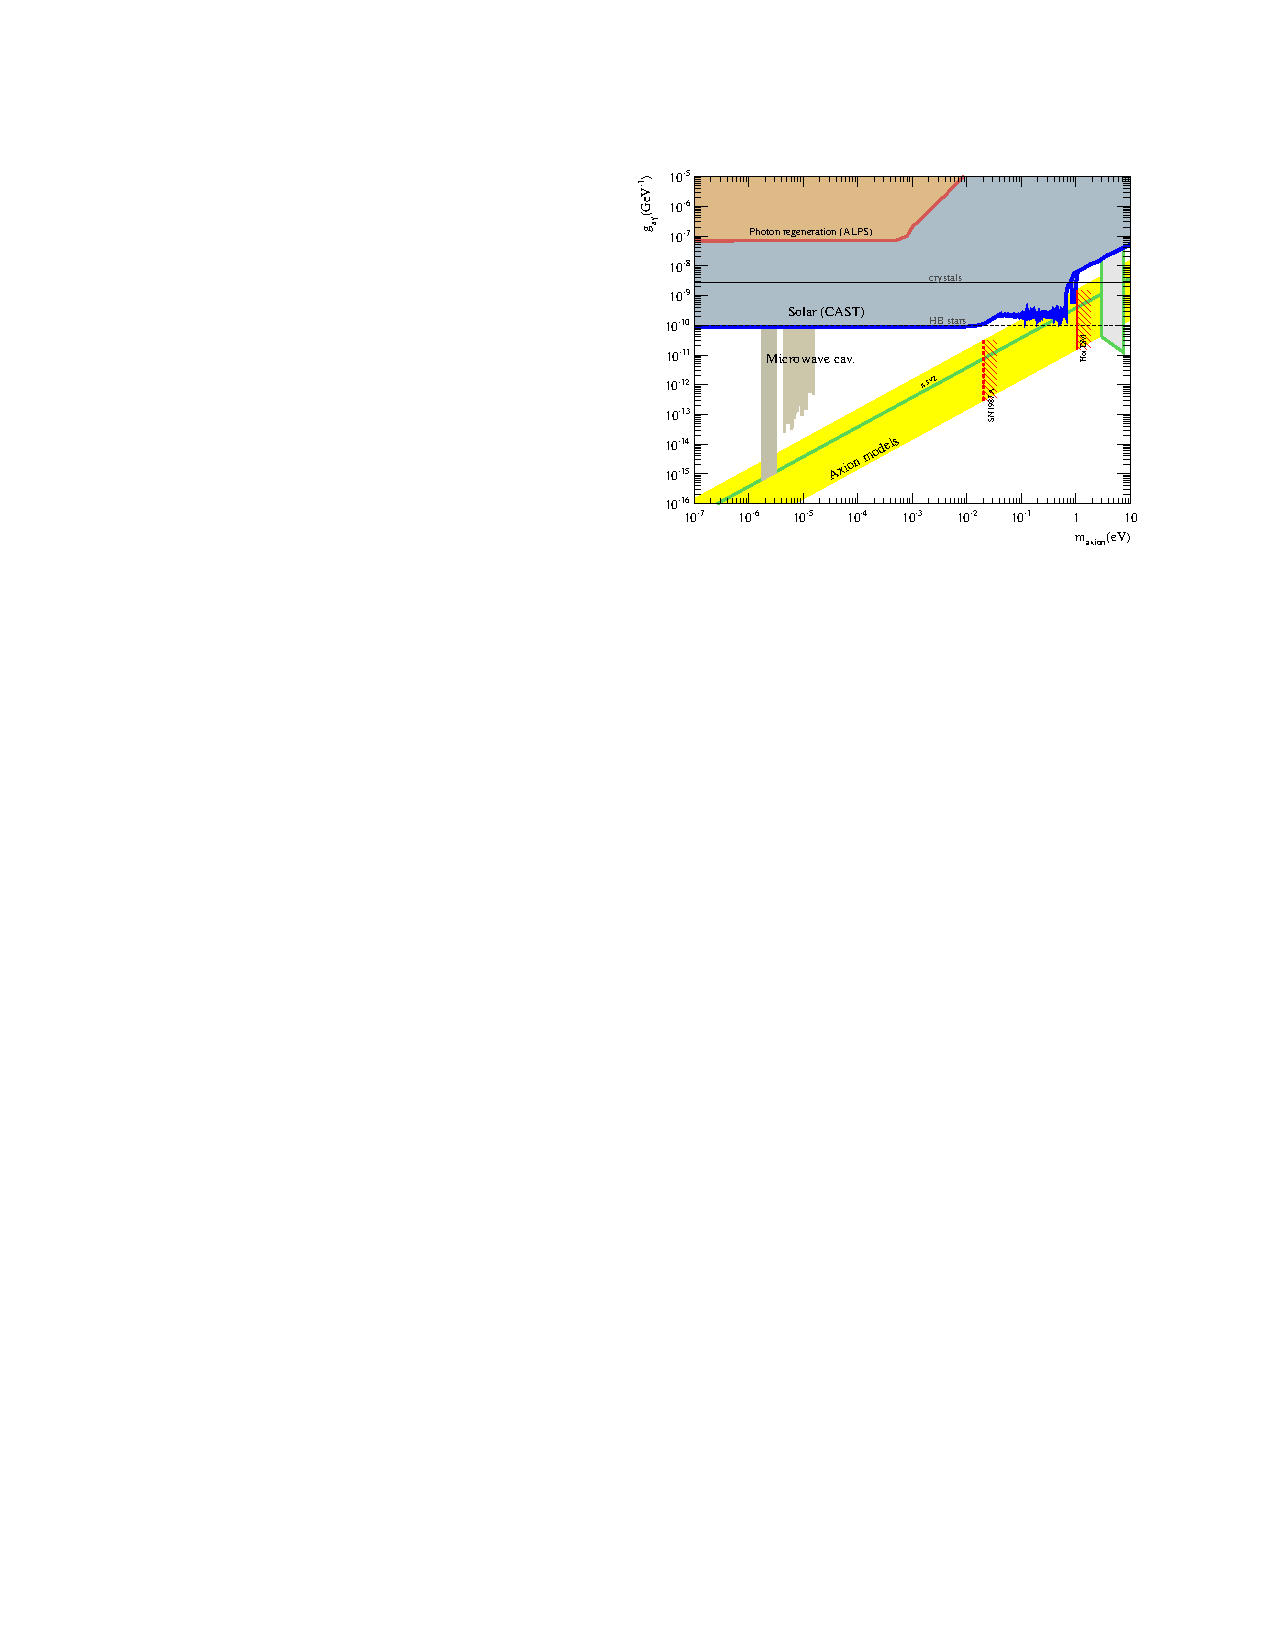
\includegraphics[width=\linewidth]{figures/cast/axion_search_cast.pdf}
  \captionof{figure}{Show bore-opening with mandrel from front.}
  \label{fig:optic_and_bore}
\end{minipage}
\end{figure}

The focal length $f$ was set to a fixed value of 1.5 m. Using $r_{\text{min}}$ as the first layer radius, $\mathit{R3}_1$, the angle of the first layer, $\alpha_1$, can be calculated using eq. \ref{eq:wolter}. From $\alpha_1$ and $\mathit{R3}_1$, we can calculate $\mathit{R1}_1$, $\mathit{R2}_1$, $\mathit{R4}_1$ and $\mathit{R5}_1$:

\begin{eqnarray}
  \mathit{R2}_1 &=& \mathit{R3}_1 + 0.5 \cdot x_{\text{sep}}\cdot\tan(\alpha),\\
  \mathit{R4}_1 &=& \mathit{R3}_1 - 0.5 \cdot x_{\text{sep}}\cdot\tan(3\alpha),\\
  \mathit{R1}_1 &=& \mathit{R2}_1 + l\cdot\sin(\alpha),\\
  \mathit{R5}_1 &=& \mathit{R4}_1 - l\cdot\sin(3\alpha),
\end{eqnarray}

where $x_{\text{sep}}$ is the distance between the parabolic and hyperbolic mirror. The next layer can be added by setting

\begin{eqnarray}
  \mathit{R3}_2 &=& \mathit{R1}_1 + d_{\text{glass}},
\end{eqnarray}

where $d_{\text{glass}}$ is the thickness of the glass. Thereby the opening will be exactly large enough for all incoming photons to hit the parabolic mirror.


!! setting the focal length to 1.5 m !!


\subsection{Optimising reflective coatings}


\section{Producing coated substrates}


\subsection{Collecting substrates for coating}

\subsection{Coating of substrates}



\section{Assembling coated substrates}


\subsection{Acquiring parts for assembly vacuum vessel}


\section{Installation of optic at CAST}


\subsection{Optic alignment}

\subsection{Tests with 8 keV X-ray source}

\section{Conclusion}
%\section{First light}
